\documentclass[uplatex, a4paper, 12pt, openany, oneside]{jsbook}

\usepackage[dvipdfmx]{graphicx}
\usepackage[dvipdfmx]{color}
\usepackage[dvipdfmx, bookmarks=true, setpagesize=false, hidelinks]{hyperref}
\usepackage{pxjahyper}

\usepackage{thesis}
\usepackage{here}
\usepackage{url}


\thesis{卒 業 論 文}
\title{
  \centering
    \scalebox{1.0}{収穫ロボット用エンドエフェクタの開発}\\
    \vspace{-0.8zh}
    \scalebox{1.0}{- 設計指標に関する検討 -}\\
    \vspace{-0.3zh}
    \scalebox{0.7}{Development of an end effector for a harvesting robot}\\
    \vspace{-0.8zh}
    \scalebox{0.7}{- Consideration of design indicators -}
    \vspace{-0.6zh}
}
\setlength{\textwidth}{\fullwidth}
\setlength{\evensidemargin}{\oddsidemargin}

\date{\today}
\vspace{-15.0zh}
\teacher{林原 靖男 教授}
\vspace{-15.0zh}
\organization{千葉工業大学 先進工学部 未来ロボティクス学科}
\author{21C1010 池田晃輝}
\vspace{-15zh}

\renewcommand{\baselinestretch}{1.2}
\begin{document}

%% Front Matter
\frontmatter{}
%
\chapter{序論}
\label{chap:introduction}
%
%\input{introduction/preface}
%
%!TEX root = ../thesis.tex

\section{背景}
農林水産省によると, 日本の農業従事者数は, 2000年から2023年にかけて約50%減少している.
また, 2023年の農業従事者のうち約7割が65歳以上の高齢者となっている.
そのため, 日本の農業分野では人手不足と高齢化による農作業の負担増大が深刻な問題となってきている.
これらの問題を解決するために作物を自動で収穫することができるロボットの開発が望まれる.
収穫ロボットに求められる技術のうちの1つに収穫用のエンドエフェクタが挙げられる.

現在, 収穫用エンドエフェクタに関する研究は多く, 既に様々なエンドエフェクタが提案されている.
%例えば, 
また, 市販されている収穫ロボットに独自のエンドエフェクタが取り付けられているものもある.
しかし, それらのエンドエフェクタの設計指針については明確に示されていない.
そのため, 収穫する作物に対して優れた形状がわからないことや, 具体的な改善点が見つけにくいことが問題となる.

Fig.?のような場合において, 赤で示されたピーマンは花柄が露出しているが果実は葉で隠れてしまっているのに対し, オレンジで示されたピーマンは花柄が葉で隠れているが果実は露出している.
赤で示されたピーマンは花柄にアプローチしやすく, オレンジで示されたピーマンは果実にアプローチしやすことがわかる.
このことから, 収穫物のいくつかの特性を定量化することで収穫物に適したエンドエフェクタの形を考える.

\subsection{RoboCup}

\begin{figure}[hbtp]
  \centering
 \includegraphics[keepaspectratio, scale=0.8]
      {images/RaspberryPiMouse.png}
 \caption{Example}
 \label{Fig:Example}
\end{figure}

\subsubsection{etc...}
\newpage

%
\section{目的}
本研究ではいくつかの収穫物周辺の特性を定量化し, その特性を用いてエンドエフェクタの設計指標を構築することを試みる.
さらに, 従来から提案されているエンドエフェクタを参考にしてエンドエフェクタのモデルを作成し, 模擬的な収穫の実験を行うことで, 実環境での収穫率を求める.
そして, 設計指標から求めた収穫率の予測値と実環境での収穫率を比較することで構築した設計指標の妥当性を検証する.

%
\section{従来のエンドエフェクタ}
%
\section{本論文の構成}
本論文の構成を述べる.
第1章では本研究の背景と目的について述べた.
第2章では要素技術について述べる.
第3章では設計指標の構築に必要な収穫物の特性について述べるたあと, 設計指標の構築について述べる.
第4章では収穫物の特性を測定した方法と結果について述べる.
第5章では構築した設計指標の有効性を検証するための実環境で行った実験について述べ, 成功率の比較を行う.
第6章では本論文の総括を述べる.
%
%% Main Matter
\mainmatter{}
%
\chapter{序論}
\label{chap:introduction}
%
%\input{introduction/preface}
%
%!TEX root = ../thesis.tex

\section{背景}
農林水産省によると, 日本の農業従事者数は, 2000年から2023年にかけて約50%減少している.
また, 2023年の農業従事者のうち約7割が65歳以上の高齢者となっている.
そのため, 日本の農業分野では人手不足と高齢化による農作業の負担増大が深刻な問題となってきている.
これらの問題を解決するために作物を自動で収穫することができるロボットの開発が望まれる.
収穫ロボットに求められる技術のうちの1つに収穫用のエンドエフェクタが挙げられる.

現在, 収穫用エンドエフェクタに関する研究は多く, 既に様々なエンドエフェクタが提案されている.
%例えば, 
また, 市販されている収穫ロボットに独自のエンドエフェクタが取り付けられているものもある.
しかし, それらのエンドエフェクタの設計指針については明確に示されていない.
そのため, 収穫する作物に対して優れた形状がわからないことや, 具体的な改善点が見つけにくいことが問題となる.

Fig.?のような場合において, 赤で示されたピーマンは花柄が露出しているが果実は葉で隠れてしまっているのに対し, オレンジで示されたピーマンは花柄が葉で隠れているが果実は露出している.
赤で示されたピーマンは花柄にアプローチしやすく, オレンジで示されたピーマンは果実にアプローチしやすことがわかる.
このことから, 収穫物のいくつかの特性を定量化することで収穫物に適したエンドエフェクタの形を考える.

\subsection{RoboCup}

\begin{figure}[hbtp]
  \centering
 \includegraphics[keepaspectratio, scale=0.8]
      {images/RaspberryPiMouse.png}
 \caption{Example}
 \label{Fig:Example}
\end{figure}

\subsubsection{etc...}
\newpage

%
\section{目的}
本研究ではいくつかの収穫物周辺の特性を定量化し, その特性を用いてエンドエフェクタの設計指標を構築することを試みる.
さらに, 従来から提案されているエンドエフェクタを参考にしてエンドエフェクタのモデルを作成し, 模擬的な収穫の実験を行うことで, 実環境での収穫率を求める.
そして, 設計指標から求めた収穫率の予測値と実環境での収穫率を比較することで構築した設計指標の妥当性を検証する.

%
\section{従来のエンドエフェクタ}
%
\section{本論文の構成}
本論文の構成を述べる.
第1章では本研究の背景と目的について述べた.
第2章では要素技術について述べる.
第3章では設計指標の構築に必要な収穫物の特性について述べるたあと, 設計指標の構築について述べる.
第4章では収穫物の特性を測定した方法と結果について述べる.
第5章では構築した設計指標の有効性を検証するための実環境で行った実験について述べ, 成功率の比較を行う.
第6章では本論文の総括を述べる.
%ここにディレクトリのパスを追加していく
%
\chapter{要素技術}
\label{chap:elemental}
%
\section{3Dスキャナ}
3Dスキャナは物体の形状を取得し, 3Dデータへと変換する装置である.
この装置は接触式と非接触式が存在し, 測定する物体に応じて使い分ける.
Fig.?のような非接触式3Dスキャナのハンディタイプはレーザや光を使って物体の表面をスキャンし, そのデータを3次元点群に変換する.
このようなハンディタイプは, 測定する環境が狭い場合や, 測定したい物体が複雑な構造を持つ場合でも小回りがきくため, 細かい部分まで計測できるという利点がある.
3Dスキャナは, 品質検査やリバースエンジニアリング, 文化財等をデジタルアーカイブとして保存することなど, 幅広い分野で活用されており, 物体を3Dデータ化することができる.
%
\section{Blender}
Blenderは, 3Dコンピュータグラフィックスやアニメーションを制作することができるオープンソースの3DCGソフトウェアである.
モデリング機能やテクスチャ機能など, 豊富な機能が備わっている.
また, Blender内に独立したPython環境が搭載されており, Python言語を使用して独自のスクリプトを作成することが可能となっている.
Blenderは商用のアニメーション映画にも利用されているほか, 建築の透視図やCADにも活用されている.
%
\chapter{設計指標の構築}
\label{chap:designindex}
%
\section{設計指標}
収穫物の特性とエンドエフェクタの形状から設計指標を構築する.
設計指標は以下のように設定した.

\begin{itemize}
  \item 花柄側面障害物間距離が許容範囲内か: $d_p$ \verb|>| $l_p$
  \item 花柄アプローチ面積より花柄が露出しているか: $S_p$ \verb|>| $S_papproach$
  \item 果実側面障害物間距離が許容範囲内か: $d_fside$ \verb|>| $l_fside$
  \item 果実上面障害物間距離が許容範囲内か: $d_fabove$ \verb|>| $l_fabove$
  \item 果実下面障害物間距離が許容範囲内か: $d_funder$ \verb|>| $l_funder$
  \item 果実アプローチ面積より果実が露出しているか: $S_f$ \verb|>| $S_fapproach$
\end{itemize}
%
\section{成功率の算出}
各エンドエフェクタはそれぞれピーマンにアプローチする部分が異なるため, 必要に応じて指標を取り入れることになる.
例えば, AGRISTのLに搭載されているエンドエフェクタの場合は, 果実にアプローチを行わないため, 花柄に関わる指標しか取り入れないこととなる.
取り入れた指標をすべて満たすものを成功とし, それ以外は失敗とする.
成功率$p_h$は以下のように表す.

\vspace{10mm}
成功率$p_h$ = 指標をすべて満たすもの / 計測した収穫物の数
\vspace{10mm}

AGRISTのLに搭載されているエンドエフェクタの場合, 成功率に関わる設計指標は, 花柄側面障害物間距離が許容範囲内かというのと花柄アプローチ面積よりも花柄が露出しているかの2つである.
よって成功率は以下のようになる.

\vspace{10mm}
$p_h = p(d_p > l_p \cap S_p > S_papproach)$
\vspace{10mm}

%
%
\chapter{植物特性の計測}
\label{chap:scan}
%
\section{実験目的}
%
\section{実験装置}
以下に実験に使用した装置およびスキャンした収穫物を示す.
3Dスキャナは非接触式でハンディタイプのArtec Leoを使用した.
スキャンした収穫物は, \figref{Fig:plant}に示すようなハウス内で栽培されているピーマン株である.
また, Blenderを用いてピーマンの3Dモデルから特性を計測した.

\vspace{5mm}
\begin{figure}[H]
     \centering
     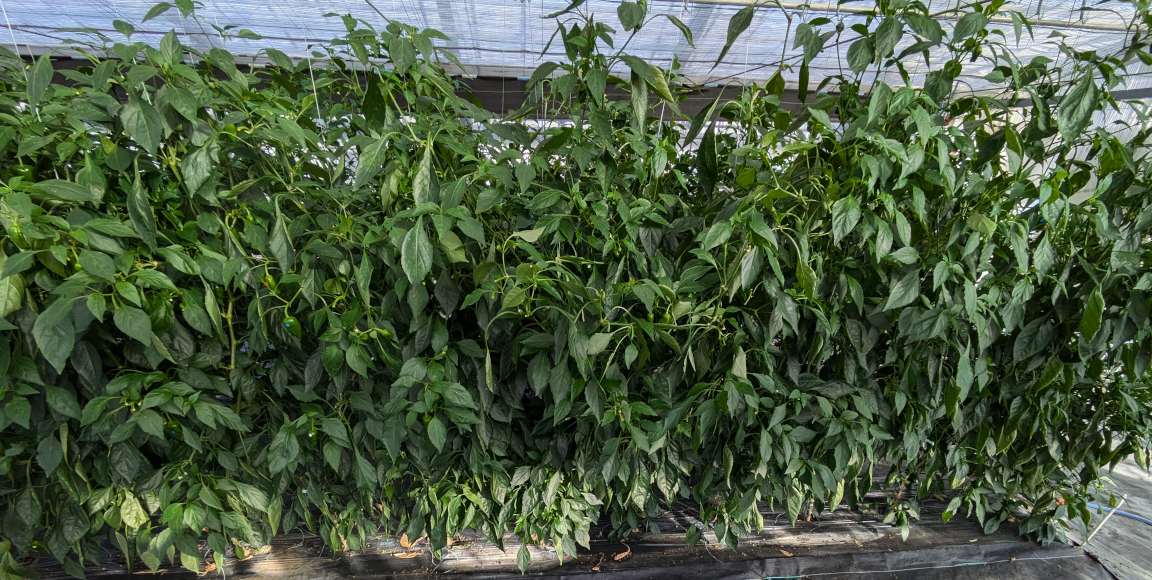
\includegraphics[width=110mm]{images/png/plant.png}
     \caption{Scanned crop}
     \label{Fig:plant}
   \end{figure}
%
\section{実験方法}
収穫物の特性を計測する手順は以下のとおりである.
計測する特性は3.1節で提案した特性と, アプローチ面積を求めるために花柄と果実の幅をそれぞれ計測する.
計測対象は30個のピーマンだが, 奥の方にあってスキャンできていないものや, 3Dモデルが大きく欠損していて計測が難しいものは計測結果からは除外する.

\begin{enumerate}
  \item 左から順に人が視認できるピーマン30個にID付け用のシールを貼る
  \item シールを貼ったピーマンがあるピーマン株に対して, Artec Leoを用いて3Dスキャンを行う
  \item 計測して得たピーマン株の3DモデルをBlender内に取り込み, 特性を計測する
\end{enumerate}

計測の例を \figref{Fig:measurement1} \verb|〜| \figref{Fig:measurement3} に示す. 
ピーマン株が複雑であることや, 3Dモデルが一部欠損している場合があり, 特性の計測を自動化することが困難だったため, 今回は手動で行った.
各障害物間距離は, 花柄と果実の内部を含まず, 花柄または果実の中心から障害物までの最小距離と思われる部分を計測した.

\vspace{5mm}
\begin{figure}[H]
     \centering
     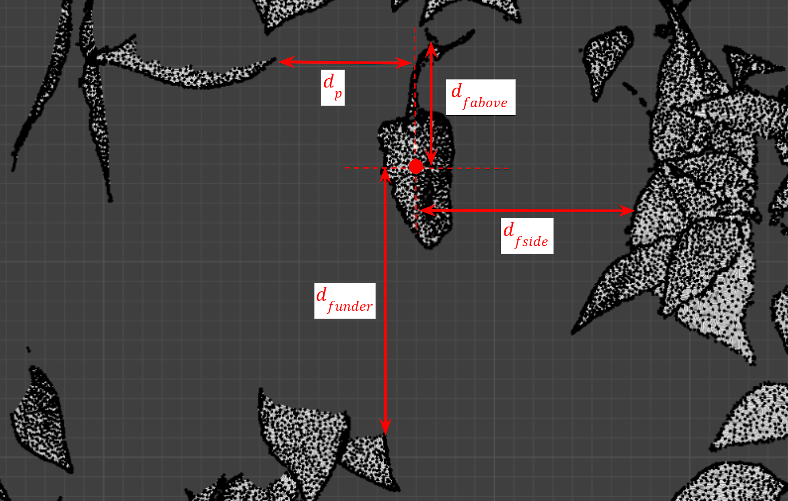
\includegraphics[width=\columnwidth]{images/png/measurement1.png}
     \caption{Measurement① distance to obstacle}
     \label{Fig:measurement1}
\end{figure}

\begin{figure}[H]
  \begin{minipage}[b]{0.48\columnwidth}
    \centering
    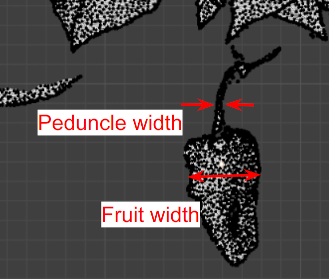
\includegraphics[width=\columnwidth]{images/png/measurement2.png}
    \caption{Measurement② width}
    \label{Fig:measurement2}
  \end{minipage}
  \hspace{0.04\columnwidth}
  \begin{minipage}[b]{0.48\columnwidth}
    \centering
    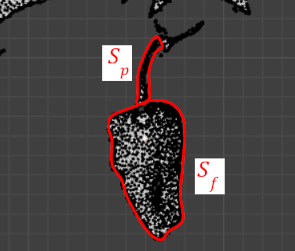
\includegraphics[width=\columnwidth]{images/png/measurement3.png}
    \caption{Measurement③ projected area}
    \label{Fig:measurement3}
  \end{minipage}
\end{figure}
%
\section{実験結果}
ピーマンの3Dモデルの計測結果は以下の通りである.
奥の方にあるピーマンは3Dスキャンが難しく, スキャンできていないことや3Dモデルが欠損している場合があり, 計測が困難だったため, 計測結果からは除外した.
%
%
\chapter{実験}
\label{chap:experiment}
%
\section{実験目的}
%
\section{実験装置}
実験装置を以下に示す.
アプローチするピーマンは前章でスキャンしたピーマンである.
\figref{Fig:finraymodel} \verb|〜| \figref{Fig:agristmodel} は作成したエンドエフェクタモデルである.
以降は, フィンレイエンドエフェクタを参考に作成したモデルをグリッパ型, 振動ナイフのエンドエフェクタを参考にしたものを振動ナイフ型, AGRISTのエンドエフェクタを参考にしたものを花柄アプローチ型と呼ぶ.
ピーマン株に対して各エンドエフェクタモデルを垂直にアプローチさせるための実験装置を \figref{Fig:device} に示す.


\vspace{5mm}
\begin{figure}[H]
     \centering
     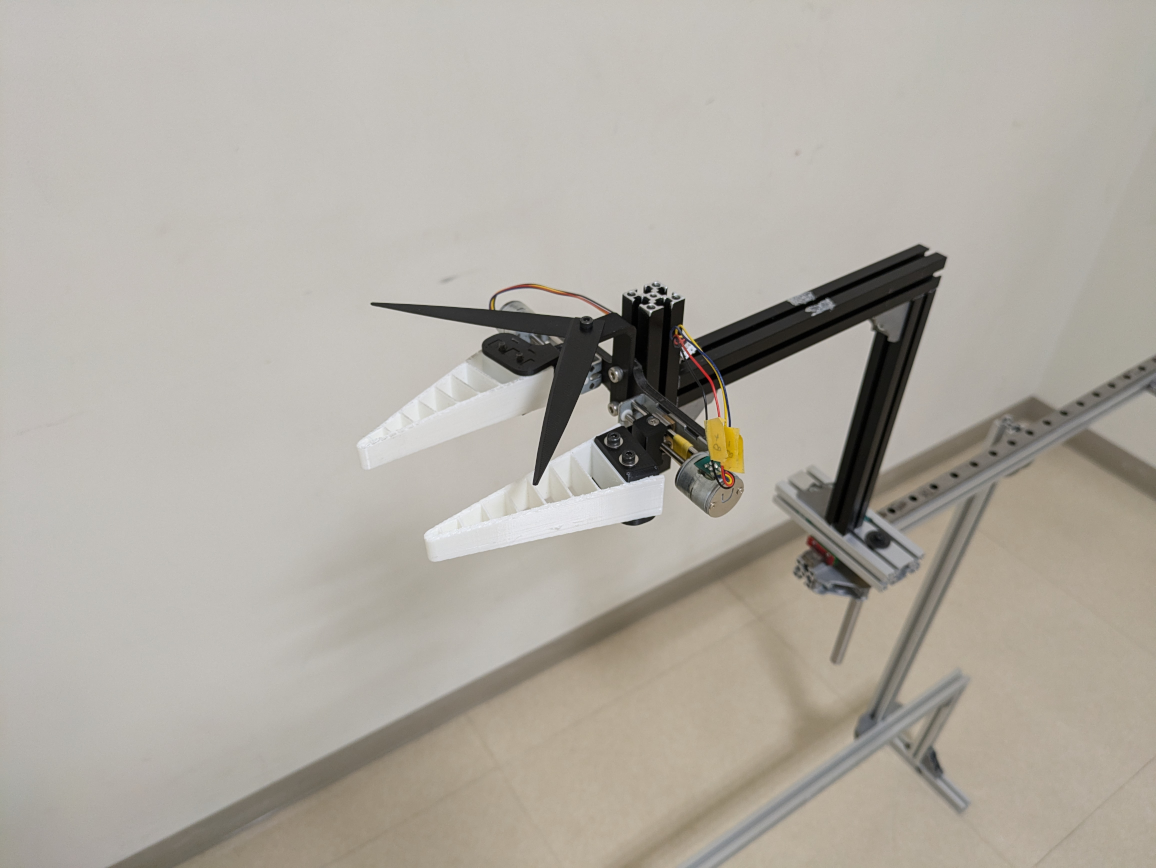
\includegraphics[width=100mm]{images/png/finray_model.png}
     \caption{end effector model① gripper type}
     \label{Fig:finraymodel}
   \end{figure}

\begin{figure}[H]
    \centering
    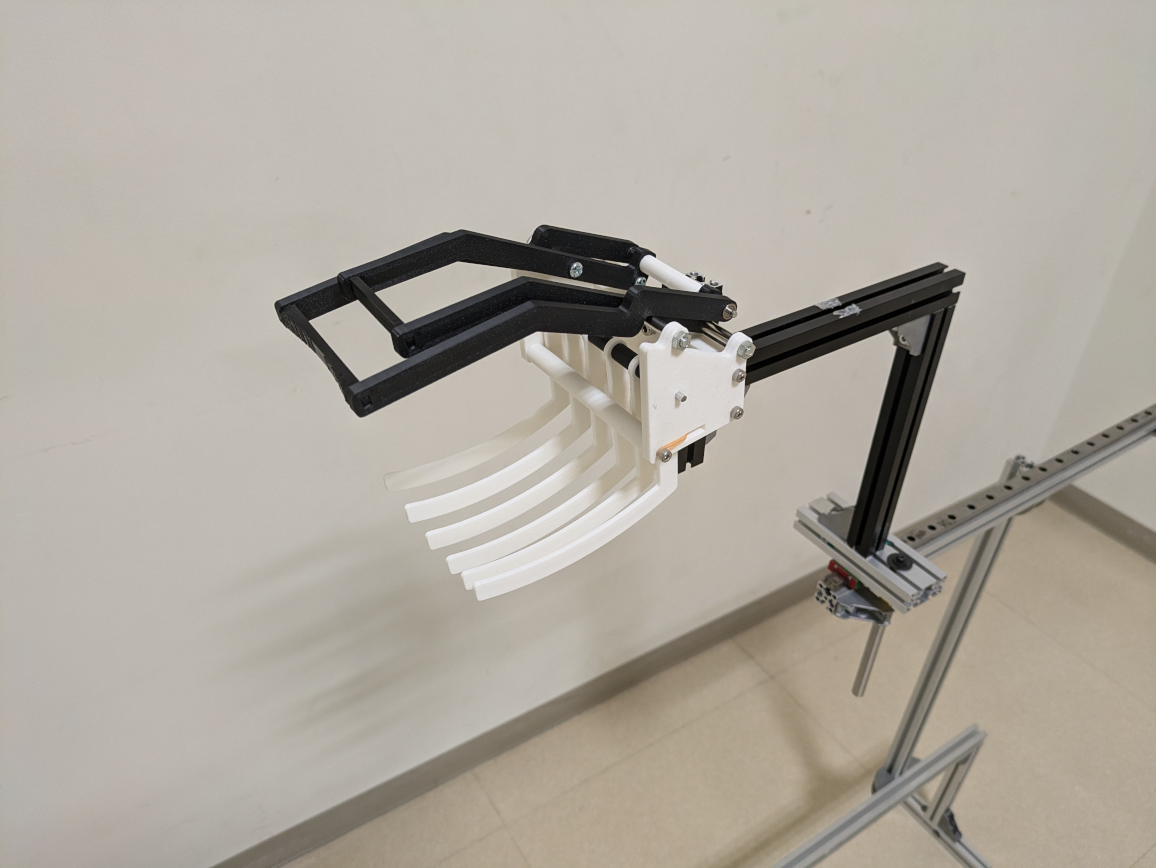
\includegraphics[width=100mm]{images/png/sweeper_model.png}
    \caption{end effector model② vibrating knife type}
    \label{Fig:sweepermodel}
   \end{figure}

\begin{figure}[H]
    \centering
    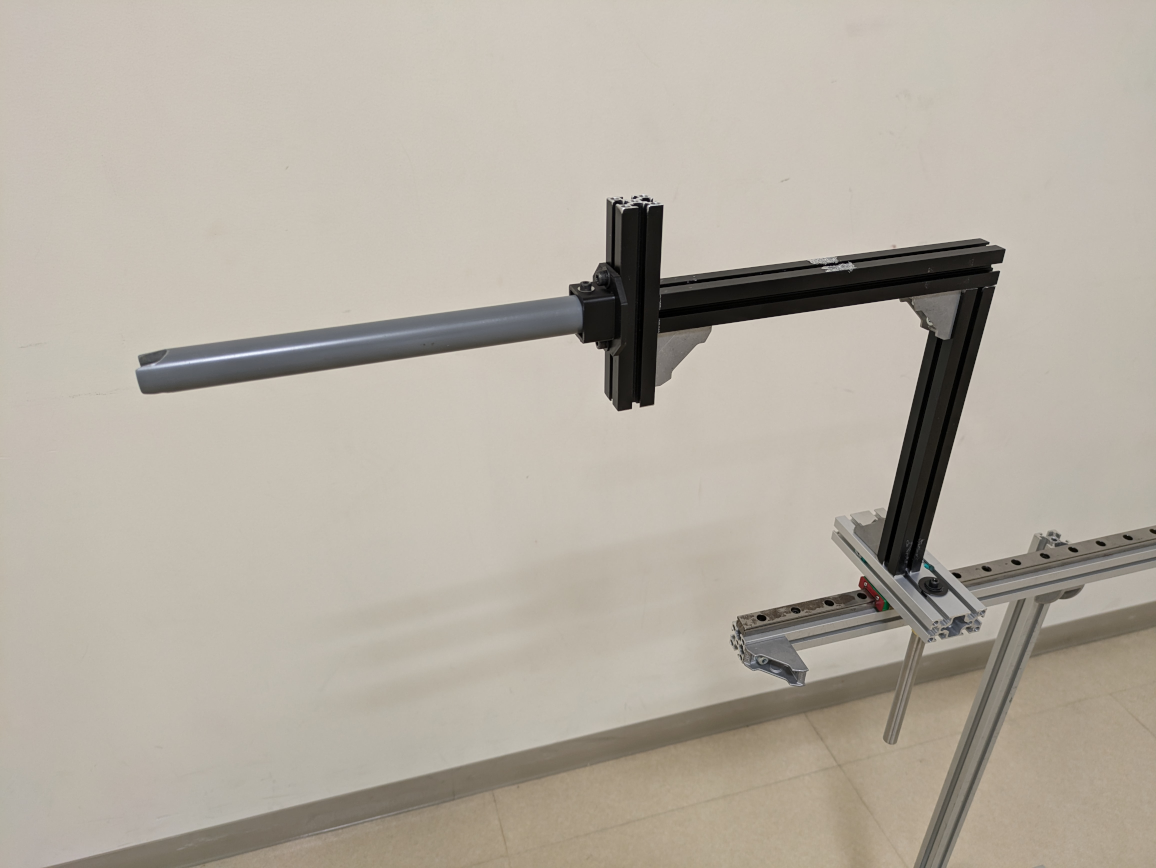
\includegraphics[width=100mm]{images/png/agrist_model.png}
    \caption{end effector model③ peduncle approach type}
    \label{Fig:agristmodel}
   \end{figure}

\begin{figure}[H]
    \centering
    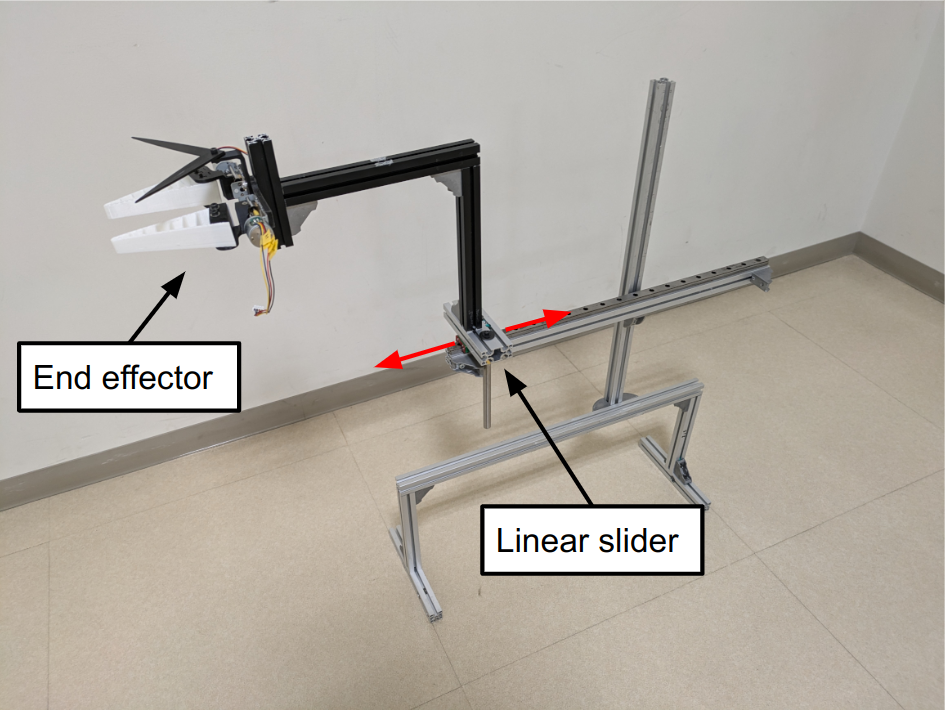
\includegraphics[width=100mm]{images/png/device.png}
    \caption{Experimental device}
    \label{Fig:device}
   \end{figure}

%
\section{実験方法}
実験手順を以下に示す. アプローチの可否は目視で判断する.
\figref{Fig:success}のようにピーマンがエンドエフェクタの収穫範囲内に入った場合は成功, \figref{Fig:failure}のように茎や葉などの収穫対象以外のものを巻き込んで把持, または切断しそうな場合は失敗とした.
\begin{enumerate}
  \item ピーマンの正面にエンドエフェクタが位置するように実験装置を配置する
  \item 実験装置をスライドさせ, ピーマン株に対して垂直方向にエンドエフェクタをアプローチさせる.
  \item アプローチの可否を判断
  \begin{description}
    \item[成功条件] ピーマンがエンドエフェクタの収穫範囲内に入った場合
    \item[失敗条件] 収穫対象以外のものを巻き込んで把持, または切断しそうな場合
  \end{description}
  \item 各エンドエフェクタモデルで手順1\verb|〜|3を30個のピーマンに対して行う
  \item 実環境での成功率と設計指標から求めた成功率を比較する
\end{enumerate}

\vspace{5mm}
\begin{figure}[H]
     \centering
     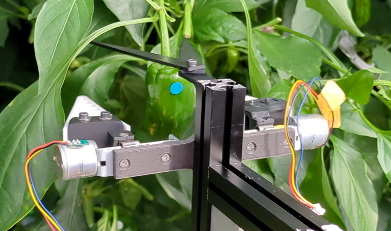
\includegraphics[width=110mm]{images/png/success.png}
     \caption{Examples of successful approaches}
     \label{Fig:success}
   \end{figure}

\begin{figure}[H]
    \centering
    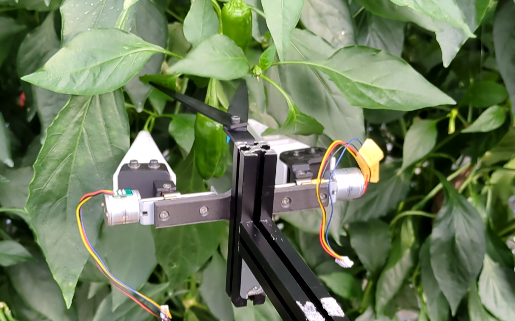
\includegraphics[width=110mm]{images/png/failure.png}
    \caption{Examples of failed approaches}
    \label{Fig:failure}
  \end{figure}
%
\section{実験結果}
\subsection{設計指標から成功率の算出}
\subsection{実環境での成功率}
\subsection{成功率の比較}
%
%
\chapter{結論}
\label{chap:conclusion}
%
\section{まとめ}
本研究では, 収穫物のいくつかの特性を定量化し, エンドエフェクタの設計指標を構築した.
また, 収穫物の3Dスキャンにより3Dモデル化して設計指標に必要な特性を計測した.
そして, 既存のエンドエフェクタを参考にモデルを作成して実際にアプローチさせることで, 設計指標の有効性を検証し, 成功率の傾向が同じであることを確認した.

%
\section{今後の展望}
%
%
%% Back Matter
\backmatter{}
%
%!TEX root = ../thesis.tex
%\bibliographystyle{plain}
\bibliographystyle{junsrt}
%\bibliography{report}
\nocite{*}
\bibliography{main_bibliography}
%
%\input{backmatter/appendix}
%
%!TEX root = ../thesis.tex
\chapter*{謝辞}
\addcontentsline{toc}{chapter}{謝辞}

本研究を進めるにあたり,1年に渡り, 熱心にご指導を頂いた林原靖男教授に深く感謝いたします.
また, 技術的な支援, ご意見を頂いたロボット設計制御研究室の皆さまや, 収穫ロボット開発チームの皆様, 共同研究者である筒井健翔氏に感謝いたします.
最後に, 日常生活を支えてくださった両親に深く感謝いたします.

%


%

\end{document}
